\newpage
\section{Measurement with back-light illumination}
There are multiple ways to measure the size and form of an object. A popular way to get the contour of an object, is to place a light source behind it and aim the camera on the object from the other side. With this method the optical sensors captures the silhouette of the object. In this section a short introduction to photometry and the typical construction of backlighting systems are discussed.
\subsection{Introduction to photometry}
Photometry is the science concerned with the electromagnetic radiation visible to the human eye. In this section, important basics used further in this thesis are explained. The theories of the following sections were taken from the textbook Physik 2 \cite{ruh}.
\subsubsection{Photometric quantities}
In principle the normal physical quantities and units, such as watts and joules, could be used for the measurements of light radiation. However, in order to take the spectral sensitivity of the human eye into account, special photometric quantities and units, displayed in Table \ref{theory:photo} are introduced.\\

\begin{table}[ht]
\centering
\begin{tabular}{ |p{6cm} p{2cm}|p{6cm} p{2cm}|  }
	\hline
	\multicolumn{2}{|c}{Quantity}&\multicolumn{2}{|c|}{Unit} \\
	\hline\hline
	\multicolumn{1}{|c}{Name}			& \multicolumn{1}{|c|}{Symbol}	& \multicolumn{1}{c}{Name}	& \multicolumn{1}{|c|}{Symbol}	\\

	\hline
	Luminous flux		& \multicolumn{1}{|c|}{$\Phi_v$}	& lumen		& \multicolumn{1}{|c|}{lm}\\
	Luminous intensity 	& \multicolumn{1}{|c|}{$I_v$} 		& candela	& \multicolumn{1}{|c|}{cd}\\
	Luminance			& \multicolumn{1}{|c|}{$L_v$}		& candela/$\text{m}^2$	& \multicolumn{1}{|c|}{cd/$\text{m}^2$}\\
	Illuminance 		& \multicolumn{1}{|c|}{$E_v$} 		& lux (lumen/$\text{m}^2$) 	& \multicolumn{1}{|c|}{lx}\\

	\hline
\end{tabular}
\caption{Photometric quantities and units. \label{theory:photo}}
\end{table}

\subsubsection{Light source}
The light source is assumed as a point which emits light in all directions.
The radiated light rays are measured in luminous flux. The density of the light rays and the luminous intensity are inversely proportional to the squared distance $r$.
This behavior has to do with the fact that the surface area $A$ of a sphere
\begin{align*}
A=\int_{0}^{2 \pi} \int_{0}^{\pi} r^{2} \sin \theta \text{d} \theta \text{d} \varphi=4 \pi r^{2}
\end{align*}
grows squared with the it's radius $r$, while the luminous flux remains constant.
This is illustrated in Figure \ref{theory:light}.
\begin{figure}[ht]
	\centering
	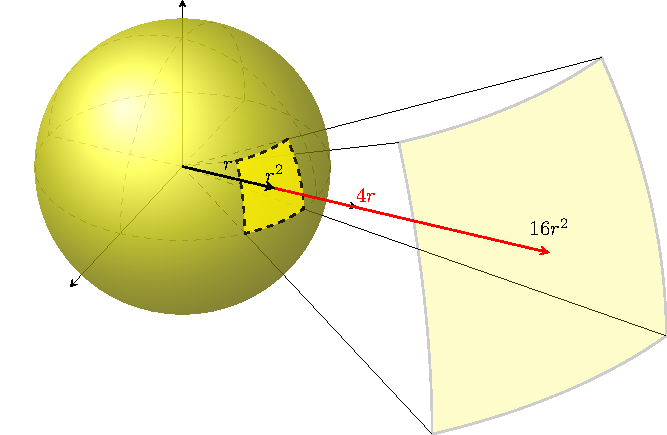
\includegraphics[width=0.6\textwidth]{2-theory/backlight/light.pdf}
	\caption{Light source in 3D.\label{theory:light}}
\end{figure} 

\subsubsection{Solid angle}
In photometry, the usage of the so-called solid angle is very common.
A beam of rays emanates from a point. The area of a sphere with radius one and the same point in it's center, which is illuminated is called the solid angle $\Omega$.
%If spherical coordinates (with $r$, $\theta$ and $\varphi$) are used, a differential solid angle element $\text{d} \Omega$ can be expressed as
%\begin{align*}
%\text{d} \Omega=\sin(\theta) \text{d} \theta\text{d} \varphi.
%\end{align*}
%The differential solid angle element can now be integrated to obtain a surface-area, with $\hat{r}$ being the unit vector of the radius
%\begin{align*}
%\Omega=\iint_{S} \frac{\hat{r} \cdot \hat{n} \text{d} S}{r^{2}}=\iint_{S} \sin \theta \text{d} \theta \text{d} \varphi.
%\end{align*}
%When defining the solid angle, a sphere with any radius $r$ can be used instead of the unit sphere. The area A cut out by the beam of rays on the surface of the sphere must then be divided by $r^2$
%\begin{align*}
%\Omega=\frac{A}{r^{2}}.
%\end{align*}
%One can see from this definition, that the solid angle is a dimensionless quantity.
\subsubsection{Luminous flux}
Luminous flux has the unit lumen (lm) and is used to describe the total amount of light a lamp emits.
The Table \ref{theory:lumflux} shows some examples, to give a better understanding of how bright a lumen really is.
\begin{table}[ht]
\begin{tabular}{ |p{12cm}| p{2cm}|  }
	\hline
	& $\Phi_v$ in lm\\
	
	
	\hline
	LED		& 500\\
	Light bulb, 220 V, 60W		& 730\\
	Light bulb, 220 V, 100W		& 1'380\\
	Fluorescent tube, 220 V, 40W		& 2'300\\
	Mercury vapor lamp, 220 V, 125W		& 5'400\\
	Mercury vapor lamp, 220 V, 2000W		& 125'000\\
	\hline
\end{tabular}
\caption{Examples of values in lumen.\label{theory:lumflux}}
\end{table}

\subsubsection{Luminous intensity}
Luminous intensity or candela is the luminous flux divided by the solid angle.
If the light beam is now focused onto one steradian (solid angle $\Omega = 4\pi$), this beam would be 10 candela.

\subsubsection{Luminance}
Luminace $L_v$ is the luminous intensity per area of the illuminated area. It is often used to measure reflections or emissions from flat and diffuse surfaces.
For a human it describes how bright a surface appears.
%\begin{align*}
%L_{\mathrm{v}}=\frac{\mathrm{d}^{2} \Phi_{\mathrm{v}}}{\mathrm{d} \Sigma \mathrm{d} \Omega_{\Sigma} \cos \theta_{\Sigma}}
%\end{align*}\\
%where $\mathrm{d}^{2} \Phi_{\mathrm{v}}$ is the luminous flux leaving the infinitesimal area $d\Sigma$ inside the infinitesimal solid angle $d\Omega_\Sigma$ with the angle $\theta_{\Sigma}$ between the normal $\mathbf{n}_{\Sigma}$ and the surface $d\Sigma$ in specified direction. \\
The Table in \ref{theory:luminance} lists some examples to get a better understanding how bright a surfaces appears.
\begin{table}[ht]
\begin{tabular}{ |p{11cm}| p{3cm}|  }
	\hline
	& $L_v$ in c/$\text{m}^2$\\
	
	
	\hline
	Computer display					& $50...300$\\
	Fluorescent tube					& $10^4$\\
	Frosted light bulb					& $10^4...10^5$\\
	Tungsten filament of a light bulb	& $10^7...2\cdot 10^7$\\
	Arc lamp							& $1.5\cdot10^8...1.8\cdot10^8$\\
	High pressure mercury lamp			& $2.5\cdot10^8...10^9$\\
	Sun									& $1.2\cdot10^9$\\
	Xenon high pressure lamp			& $10^9...10^10$\\
	
	\hline
\end{tabular}
\caption{Examples of surfaces with different luminances.\label{theory:luminance}}
\end{table}

\subsubsection{Illuminance}
Illuminance describes the the total luminous flux per area. It is also known as lux (lx) or lumen per square meter.
It should not be called brightness to prevent confusion with other quantities as mean luminace.
Some examples of illuminance are in the following table.
\begin{table}[ht]
\begin{tabular}{ |p{11cm} |p{3cm}|  }
	\hline
	& $E_v$ in lx\\
		
	\hline
	Sun light in summer					& 70'000\\
	Sun light in winter					& 5'500\\
	Day light with clouded sky			& 1'000-2'000\\
	Full moon night						& 0.25\\
	Stars without moon clear sky		& 0.001\\
	Limit of color perception			& 3\\
	Streetlight							& 1-30\\
	Living room							& 40-150\\
	Working room						& 40-300\\
	Working place lightning				& 100-4000\\
	
	\hline
\end{tabular}
\caption{Examples of different illuminances.\label{theory:illuminance}}	
\end{table}

%Since the quantities used in photometry are only in the light frequency spectrum see able by the human eye, here is a comparison of the radiometry quantities and the photometry quantities.

%\begin{tabular}{ |p{4cm} p{2cm} p{2cm}|p{4cm} p{2cm} p{2cm}|  }
%		\hline
%		\multicolumn{3}{|c}{Radiometry}&\multicolumn{3}{|c|}{Photometry} \\
%		\hline\hline
%		\multicolumn{1}{|l}{Name}			& \multicolumn{1}{c}{Symbol}& \multicolumn{1}{c|}{Unit}	& \multicolumn{1}{c}{Name}	& \multicolumn{1}{c}{Symbol}	& \multicolumn{1}{c|}{Unit}\\
%		\hline
%		Radiant flux			& \multicolumn{1}{|c|}{$\Phi_e$}&  \multicolumn{1}{|c|}{W}		& Luminous flux		& \multicolumn{1}{|c|}{$\Phi_v$}	&  \multicolumn{1}{|c|}{lm}\\
%		Radiant intensity		& \multicolumn{1}{|c|}{$I_e$}	&  \multicolumn{1}{|c|}{W/sr}	&Luminous intensity 	& \multicolumn{1}{|c|}{$I_v$} 		&  \multicolumn{1}{|c|}{cd}\\
%		Radiace					& \multicolumn{1}{|c|}{$L_e$}	&  \multicolumn{1}{|c|}{W/$m^2$sr}		&Luminance			& \multicolumn{1}{|c|}{$L_v$}		&  \multicolumn{1}{|c|}{cd/$m^2$}\\
%		Irradiance flux density	& \multicolumn{1}{|c|}{$E_e$}	&  \multicolumn{1}{|c|}{W/$m^2$}		&Illuminace 			& \multicolumn{1}{|c|}{$E_v$} 		&  \multicolumn{1}{|c|}{lx}\\
%		
%		\hline
%\end{tabular}

\subsection{Backlight illumination}
The principle of backlight illumination is straight forward.
By placing an object in front of an light source the camera captures the silhouette of the object.
This is shown in Figure \ref{theory:backlight}.
\begin{figure}[ht]
	\centering
	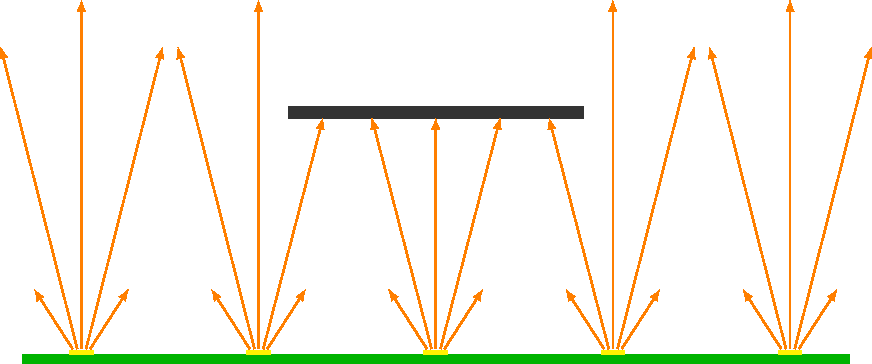
\includegraphics[width=0.9\linewidth]{2-theory/backlight/object.pdf}
	\caption{Principle of the backlight illumination.\label{theory:backlight}}	
\end{figure}

Each infinitesimal area of the backlight-surface is a light source, from which light rays spread in all directions.
If an object is now placed right on the backlight, it is possible that the object displays shade effects on the edges.
This happens because the light points on the side of the backlight - illuminating the objects surface from the side - and not only from the back. 

In Figure \ref{theory:close} the effect of the shaded edges can be clearly seen.
To reduce this effect, the object can be placed further away from the light source.
This enhances the contrast.
In Figure \ref{theory:far} the backlight is placed 8\,cm away which, leads to less stray light and sharper edges.

\begin{figure}[ht]
	\centering
	\subfigure[Backlight close to object \cite{screw1}.\label{theory:close}]{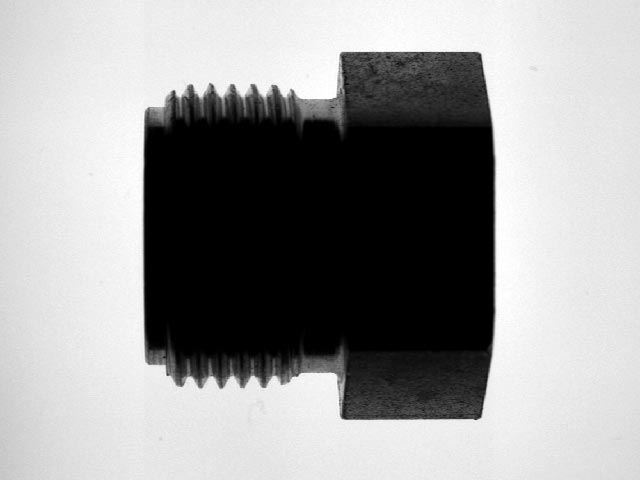
\includegraphics[width=0.45\linewidth, height=5cm]{2-theory/backlight/Schraube_durchlicht_direkt_aufgelegt.jpg}}
	\subfigure[Backlight placed 8\,cm away \cite{screw2}.\label{theory:far}]{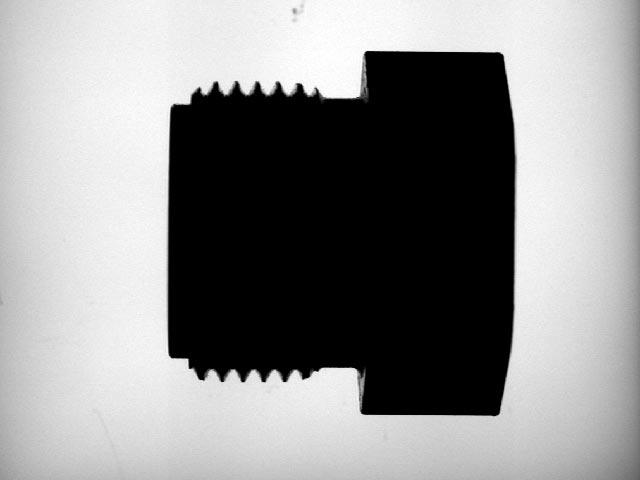
\includegraphics[width=0.45\linewidth, height=5cm]{2-theory/backlight/Schraube_durchlicht_weit_aufgelegt.jpg}}
	\caption{Comparison of different object to backlight distances.\label{theory:thre}}	
\end{figure}

Another way to control stray light is to work with so called light control filters.
These filters are build in a way, so that only light rays orthogonal to the filter can pass, thus removing the stray light from the side, resulting in much sharper edges.
Figure \ref{theory:filter} shows the effect of such a filter.
\begin{figure}[ht]
	\centering
	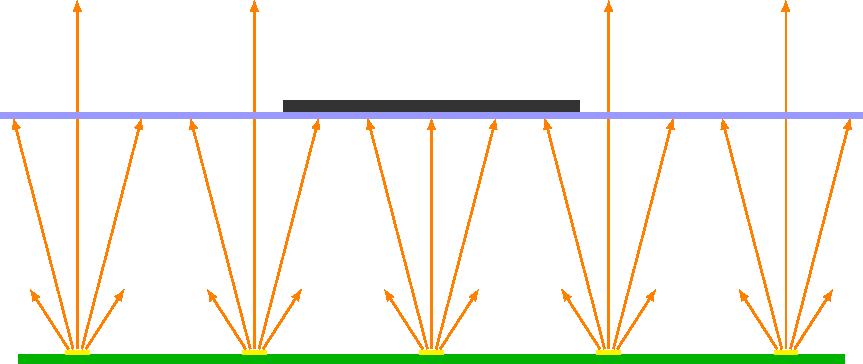
\includegraphics[width=0.9\linewidth]{2-theory/backlight/object_filter.pdf}
	\caption{Principle of a light control filter.\label{theory:filter}}	
\end{figure}

The disadvantage of this method is that the luminance after is lower than before the filter.
This leads to a darker image and makes use of an even brighter backlight necessary.
This effect is visible in Figure \ref{theory:filtercompare}.
\begin{figure}[ht]
	\centering
	\subfigure[Without filter \cite{filter1}.\label{theory:filter1}]{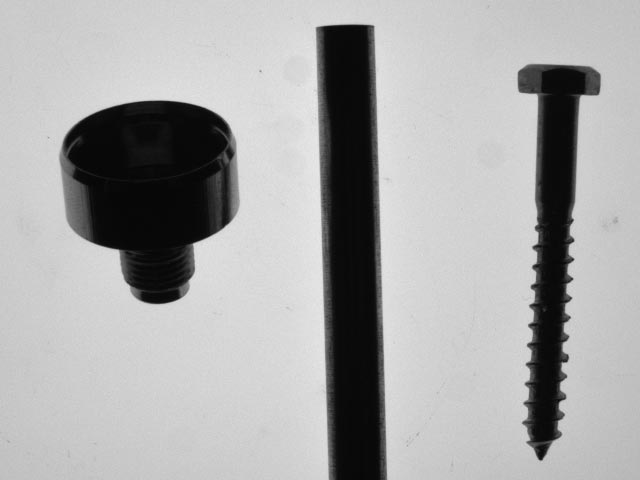
\includegraphics[width=0.45\linewidth, height=5cm]{2-theory/backlight/Durchlicht_ohne_LightControl_Filter.jpg}}
	\subfigure[With filter \cite{filter2}.\label{theory:filter2}]{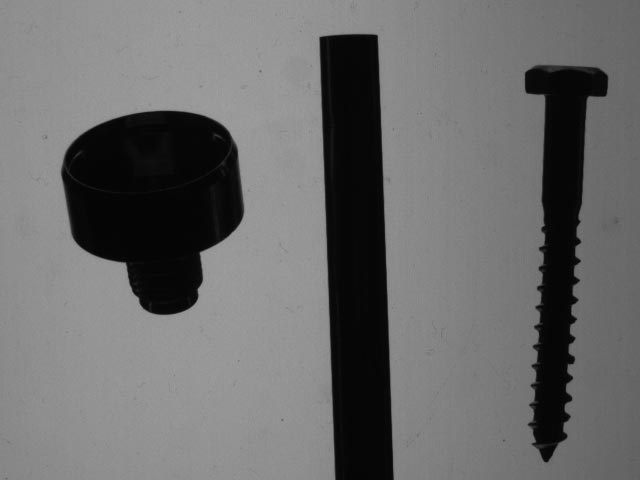
\includegraphics[width=0.45\linewidth, height=5cm]{2-theory/backlight/Durchlicht_mit_LightControl_Filter.jpg}}
	\caption{Light control filter.\label{theory:filtercompare}}	
\end{figure}

